\documentclass[a4paper,14pt]{article}
\usepackage{blindtext}
\usepackage[T2A]{fontenc}
\usepackage[utf8]{inputenc}
\usepackage[english,russian]{babel}
\usepackage{listings}
\usepackage{geometry}
\usepackage{amssymb}
\usepackage{amsmath}
\usepackage[14pt]{extsizes}
\geometry{left=3cm}
\geometry{right=1.5cm}
\geometry{top=2cm}
\geometry{bottom=2cm}
\pagestyle{plain}
\usepackage{pgfplots}
\usepackage{filecontents}
\usepackage{graphicx}
\usepackage{indentfirst}
\DeclareGraphicsExtensions{.png}
\graphicspath{{images/}}
\usetikzlibrary{datavisualization}
\usetikzlibrary{datavisualization.formats.functions}
\usepackage{tabularx}
\pgfplotsset{width=7 cm}
\usepackage{xcolor}
%\renewcommand{\rmdefault}{ftm}
%\usepackage{mathptmx}
\usepackage{setspace}
%\usepackage{minted}
%\полуторный интервал
\onehalfspacing
\frenchspacing

\usepackage{tocloft}
\frenchspacing
\setcounter{page}{3}
\usepackage{multirow}
\usepackage{float}
\usepackage{multirow}

\renewcommand{\cftsecdotsep}{\cftdot}
\renewcommand{\cftsecleader}{\cftdotfill{\cftsecdotsep}}
\renewcommand{\cftsubsecleader}{\cftdotfill{\cftsecdotsep}}
\renewcommand{\cftsubsubsecleader}{\cftdotfill{\cftsecdotsep}}

%\renewcommand\cftchapdotsep{\cftdot}
%\renewcommand\cftsecdotsep{\cftdot}
%\renewcommand{\cftchapleader}{\cftdotfill{\cftchapdotsep}}

% Для измененных титулов глав:
% % подключаем нужные пакеты
%\definecolor{gray75}{gray}{0.75} % определяем цвет
%\newcommand{\hsp}{\hspace{20pt}} % длина линии в 20pt
% titleformat определяет стиль
%\titleformat{\chapter}[hang]{\Huge\bfseries}{\thechapter\hsp\textcolor{black}{|}\hsp}{0pt}{\Huge\bfseries}
%\usepackage{titlesec, blindtext, color}
%\titleformat{\chapter}[hang]{\Huge\bfseries}{\thechapter\hsp\textcolor{black}{|}\hsp}{0pt}{\Huge\bfseries}

% Для листинга кода:
\lstset{ %
language=python,                 % выбор языка для подсветки
basicstyle=\small\sffamily, % размер и начертание шрифта для подсветки кода
numbers=left,               % где поставить нумерацию строк (слева\справа)
numberstyle=\tiny,           % размер шрифта для номеров строк
stepnumber=1,                   % размер шага между двумя номерами строк
numbersep=5pt,                % как далеко отстоят номера строк от подсвечиваемого кода
showspaces=false,            % показывать или нет пробелы специальными отступами
showstringspaces=false,      % показывать или нет пробелы в строках
showtabs=false,             % показывать или нет табуляцию в строках
frame=single,              % рисовать рамку вокруг кода
tabsize=4,                 % размер табуляции по умолчанию равен 2 пробелам
captionpos=t,              % позиция заголовка вверху [t] или внизу [b]
breaklines=true,           % автоматически переносить строки (да\нет)
breakatwhitespace=false, % переносить строки только если есть пробел
escapeinside={\#*}{*)},   % если нужно добавить комментарии в коде
literate={а}{{\selectfont\char224}}1
{б}{{\selectfont\char225}}1
{в}{{\selectfont\char226}}1
{г}{{\selectfont\char227}}1
{д}{{\selectfont\char228}}1
{е}{{\selectfont\char229}}1
{ё}{{\"e}}1
{ж}{{\selectfont\char230}}1
{з}{{\selectfont\char231}}1
{и}{{\selectfont\char232}}1
{й}{{\selectfont\char233}}1
{к}{{\selectfont\char234}}1
{л}{{\selectfont\char235}}1
{м}{{\selectfont\char236}}1
{н}{{\selectfont\char237}}1
{о}{{\selectfont\char238}}1
{п}{{\selectfont\char239}}1
{р}{{\selectfont\char240}}1
{с}{{\selectfont\char241}}1
{т}{{\selectfont\char242}}1
{у}{{\selectfont\char243}}1
{ф}{{\selectfont\char244}}1
{х}{{\selectfont\char245}}1
{ц}{{\selectfont\char246}}1
{ч}{{\selectfont\char247}}1
{ш}{{\selectfont\char248}}1
{щ}{{\selectfont\char249}}1
{ъ}{{\selectfont\char250}}1
{ы}{{\selectfont\char251}}1
{ь}{{\selectfont\char252}}1
{э}{{\selectfont\char253}}1
{ю}{{\selectfont\char254}}1
{я}{{\selectfont\char255}}1
{А}{{\selectfont\char192}}1
{Б}{{\selectfont\char193}}1
{В}{{\selectfont\char194}}1
{Г}{{\selectfont\char195}}1
{Д}{{\selectfont\char196}}1
{Е}{{\selectfont\char197}}1
{Ё}{{\"E}}1
{Ж}{{\selectfont\char198}}1
{З}{{\selectfont\char199}}1
{И}{{\selectfont\char200}}1
{Й}{{\selectfont\char201}}1
{К}{{\selectfont\char202}}1
{Л}{{\selectfont\char203}}1
{М}{{\selectfont\char204}}1
{Н}{{\selectfont\char205}}1
{О}{{\selectfont\char206}}1
{П}{{\selectfont\char207}}1
{Р}{{\selectfont\char208}}1
{С}{{\selectfont\char209}}1
{Т}{{\selectfont\char210}}1
{У}{{\selectfont\char211}}1
{Ф}{{\selectfont\char212}}1
{Х}{{\selectfont\char213}}1
{Ц}{{\selectfont\char214}}1
{Ч}{{\selectfont\char215}}1
{Ш}{{\selectfont\char216}}1
{Щ}{{\selectfont\char217}}1
{Ъ}{{\selectfont\char218}}1
{Ы}{{\selectfont\char219}}1
{Ь}{{\selectfont\char220}}1
{Э}{{\selectfont\char221}}1
{Ю}{{\selectfont\char222}}1
{Я}{{\selectfont\char223}}1
}


\begin{document}

\begin{titlepage}

    \begin{table}
        \centering
        \footnotesize
        \begin{tabular}{cc}
            \multirow{8}{*}{
\includegraphics[scale=0.35]{bmstu.jpg}}
             &                                                                           \\
             &                                                                           \\
             & \textbf{Министерство науки и высшего образования Российской Федерации}    \\
             & \textbf{Федеральное государственное бюджетное образовательное учреждение} \\
             & \textbf{высшего образования}                                              \\
             & \textbf{<<Московский государственный технический}                         \\
             & \textbf{университет имени Н.Э. Баумана>>}                                 \\
             & \textbf{(МГТУ им. Н.Э. Баумана)}                                          \\
        \end{tabular}
    \end{table}

    \vspace{-2.5cm}

    \begin{flushleft}
        \rule[-1cm]{\textwidth}{3pt}
        \rule{\textwidth}{1pt}
    \end{flushleft}

    \begin{flushleft}
        ФАКУЛЬТЕТ Информатика и системы управления
    \end{flushleft}
    КАФЕДРА Программное обеспечение ЭВМ и информационные технологии

    \vspace{3cm}

    \begin{center}
        \textbf{Лабораторная работа № 7} \\
        \textbf{Дисциплина: <<Экономика программной инженерии>>}
        \vspace{0.5cm}
    \end{center}


    \vspace{3cm}

    \begin{flushleft}
        \begin{tabular}{ll}
            \textbf{Студент}       & Пронин А. С., Климов И. С. \\
            \textbf{Группа}        & ИУ7-82Б           \\
            \textbf{Вариант}       & 2           \\
        \end{tabular}
    \end{flushleft}

    \vspace{3cm}

    \begin{center}
        Москва, 2023 г.
    \end{center}

\end{titlepage}

\setcounter{page}{2}

\subsection*{Подсчет количества объектных точек}

Количество простых экранных форм примем равным восьми (просмотр и оплата штрафов, регистрация, авторизация для web-приложения и мобильного приложения, просмотр всех выплат, просмотр данных пользователей, их редактирование и создание новых пользователей).

Количество модулей, написанных на ЯП третьего поколения -- пять.
\begin{enumerate}
    \item Приложение для мобильного телефона
    \item Веб-портал
    \item Модуль регистрации и авторизации
    \item Модуль обмена данными с системой ГИБДД
    \item Модуль проведения платежных транзакций
\end{enumerate}

\begin{table}[H]
\begin{tabular}{|l|l|l|l|}
\hline
Наименование объекта & Уровень сложности & Количество & Число точек \\ \hline
Форма                & Низкий (1)        & 12          & 12           \\ \hline
Модуль               &                   & 5          & 50          \\ \hline
Всего                &                   & 17         & 62          \\ \hline
\end{tabular}
\end{table}

Итоговое кол-во объектных точек - 62. Кол-во новых оъектных точек - 62, так как RUSE = 0.

\subsection*{Подсчет количества функциональных точек}

В  ПО имеется  два  внутренних  логический  файла  (ILF). 

Один для хранения  информаци о пользователях. Число типов элементов записей (RET) для этого файла равно двум (id - число, все остальное - строки). Число  типов  элементов  данных  (DET)  внутреннего  логического файла  будет  равно шести. Таким  образом,  уровень  сложности  внутреннего логического файла – низкий.

Второй для хранения  платежных транзакций. ILF имеет четыре элемента данных. Число типов элементов записей равно двум. Уровень сложности низкий.

ПО имеет один внешний интерфейсный файл для хранения штрафов. Число типов элементов записей (RET) для этого файла равно трем. Число  типов  элементов  данных  (DET)  внутреннего  логического файла  будет  равно шести. Таким  образом,  уровень  сложности  внутреннего логического файла – низкий.

Внешние вводы ПО:

\begin{itemize}
    \item Регистрация (мобильное приложение и веб портал). Ссылается на один внутренний логический файл и имеет пять элементов данных. Уровень сложности - низкий.
    \item Авторизация (мобильное приложение и веб портал). Ссылается на один внутренний логический файл и имеет три элемента данных. Уровень сложности - низкий.
    \item Оплата штрафа (мобильное приложение и веб-портал). Ссылается на один внешний интерфейсный файл, один внутренний логический файл и имеет пять элементов данных. Уровень сложности средний.
    \item Добавление пользователей в БД (веб-портал). Ссылется на один внутренний логический файл и имеет четыре элемента данных. Уровень сложности низкий.
    \item Получение списка штрафов (веб-портал). Ссылается на один внешний интерфейсный файл и имеет шесть элементов данных. Уровень сложности низкий.
    \item Получение сообщения об успешном или неуспешном оплате штрафа от ГИБДД (веб-портал). Имеет один элемент данных и не ссылается на внутренние файлы. Уровень сложности низкий.
    \item Ответ о результате оплаты от платежной системы (веб-портал). Имеет один элемент данных и ссылается на один внутренний файл. Уровень сложности низкий.
\end{itemize}

Внешние выводы ПО:

\begin{itemize}
    \item Вывод сообщения о положительном или отрицательном результате авторизации (веб портал + мобильное приложение). Уровень  сложности  этого внешнего вывода – низкий, так как он имеет один DET и не имеет FTR.
    \item Вывод сообщения о положительном или отрицательном результате оплаты штрафа (веб портал + мобильное приложение). Уровень  сложности  этого внешнего вывода – низкий, так как он имеет один DET и один FTR.
    \item Вывод списка штрафов.  Ссылается на один внешний интерфейсный файл и имеет один элемент данных. Уровень сложности низкий.
    \item Оповещение ГИБДД об оплате штрафа (веб-портал). Ссылается на один внутренний логический файл и имеет один элемент данных. Уровень сложности низкий.
    \item Запрос об оплате штафа (веб-портал). Имеет три элемента данных и ссылается на два внутренних файла. Уровень сложности низкий.
\end{itemize}

\begin{table}[H]
\begin{tabular}{|l|l|l|l|l|}
\hline
                            & Низкий & Средний                  & Высокий                  & Итого \\ \hline
Вневшние вводы              & 9*3    & 1*6                      & 0*4                      & 33    \\ \hline
Внешние выводы              & 5*4    & 0*5                      & 0*7                      & 20    \\ \hline
Внешние запросы             & 0*3    & {0*4} & {0*6} & 0     \\ \hline
Внутренний логический файлы & 2*7    & 0*10                     & 0*15                     & 14    \\ \hline
Внешние логический файлы    & 1*5    & 0*7                      & 0*10                     & 5    \\ \hline
Всего    &     &                      &                    & 72    \\ \hline
\end{tabular}
\end{table}

Итоговое кол-во функциональных точек - 72. Скорректированное количество функциональных точек равно 77.04.

С учетом выбранных ЯП, итоговое кол-во строк кода равно 3944.

Показатель степени равен $1.01 + (6.2+5.07+1.41+1.1+4.68) / 100)$, то есть $1.19$.

Ввод данных для метода функциональных точек представлен на рисунке \ref{fig:fp_set}. Ввод данных для методики COCOMO2 и результаты рассчетов представлены на рисунке \ref{fig:input1}. 

\newpage
\begin{figure}[!h]
    \center{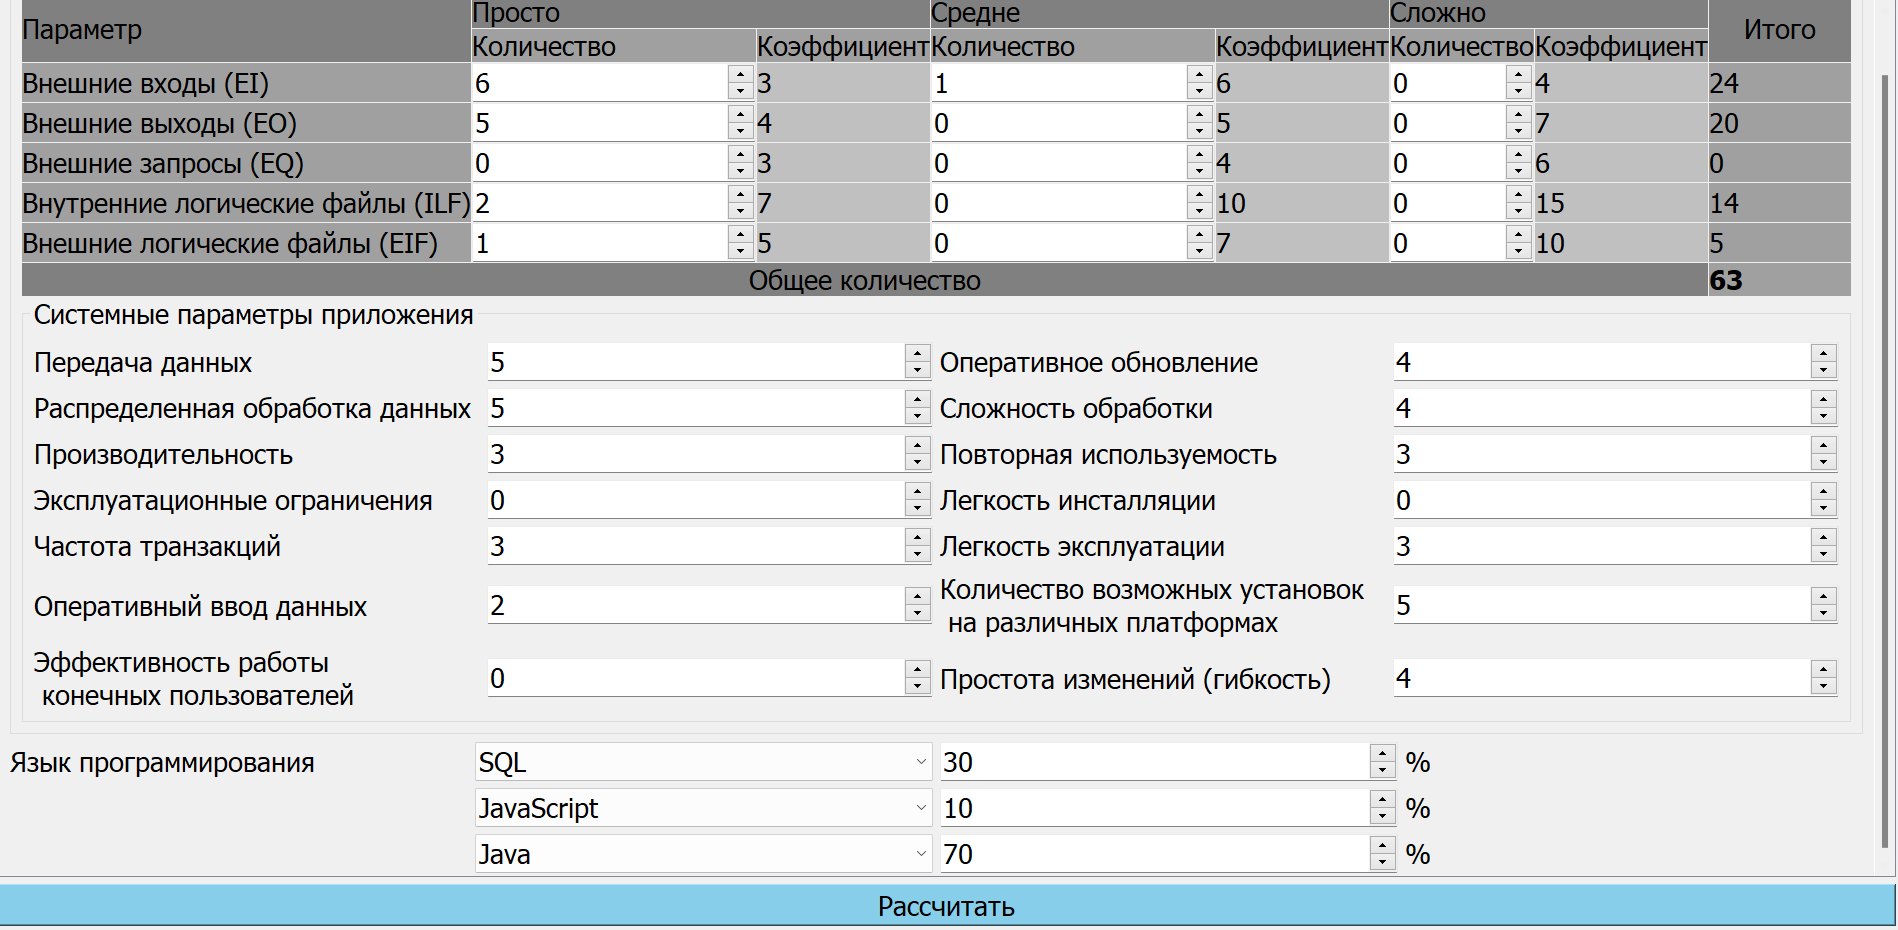
\includegraphics[width=16cm]{fp_set}}     \caption{Ввод данных для метода функциональных точек.}
    \label{fig:fp_set}
\end{figure}

\newpage
\begin{figure}[!h]
    \center{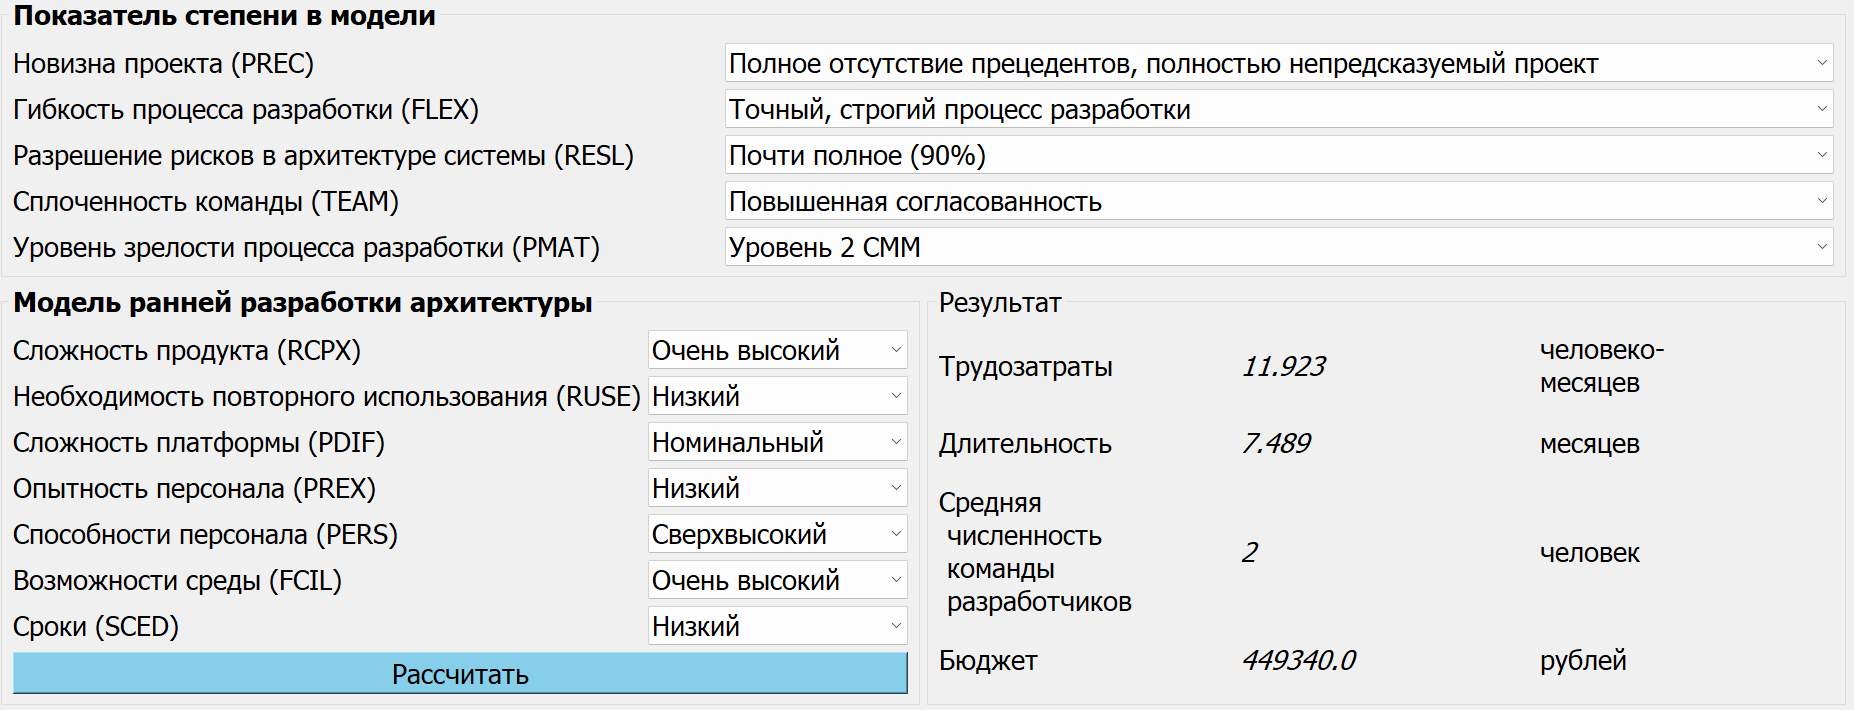
\includegraphics[width=16cm]{input1}}     \caption{Ввод данных для методики COCOMO2 (часть1).}
    \label{fig:input1}
\end{figure}

\subsection*{Вывод}

Модель COCOMO2 позволяет более полно учитывать факторы, влияющих на экономические характеристики производства сложных программных продуктов, а также учитывать уникальные факторы для корректировки экономических характеристик, связанные со специфическим проектом и организацией.

COCOMO2 и метод функциональных точек предоставляет возможность оценить объем проекта если собственный опыт аналогичных проектов отсутствует, а экспертное мнение недоступно.

\end{document}
